\chapter{Weights}
\label{chapter:weights}

\section{Introduction}
\label{section:introduction}
The first task set is concerned with the transport of goods and of key importance in information technology and finds various application fields. Associated to this task is a well-known problem in the field called 'rucksack problem'. The tasks modelled here are simplified and do not require the solution to fulfil as many conditions as in the rucksack problem. 

In this task set, different weights, labelled with 1 to 12 kilograms (see figure \ref{fig:weights}), are available and can be distributed among boats of different capacities (see figure \ref{fig:boats}). Throughout the levels, the user has to check and distribute the weights. The condition for a solution to be valid is that all weights of the initial weight set are used and that no boat is overloaded.


\begin{figure}[H]
    \centering
    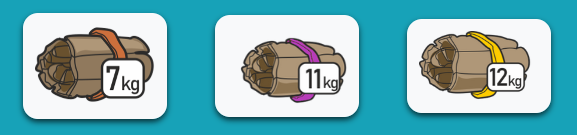
\includegraphics[width=0.6 \columnwidth]{figures/weights.png}
    \caption{Weights of Different Sizes} 
    \label{fig:weights} 
\end{figure}

\begin{figure}[H]
    \centering
    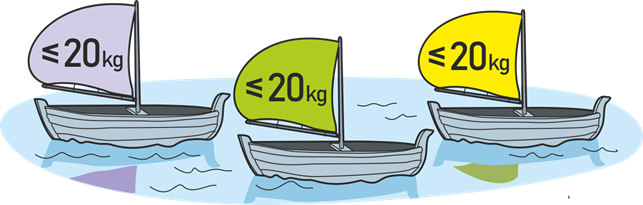
\includegraphics[width=0.6 \columnwidth]{figures/boats.png}
    \caption{Boats with Weight Capacities} 
    \label{fig:boats} 
\end{figure}

\section{Levels and Goals}
\label{section:assignment}

The goal of this exercise set is to train the competence to plan and conduct transports of a given quantity while minimizing the effort and resources assigned to it. 

On the first level, the students are required to observe all the given weights closely. There may be weights that have not been distributed in spite of being on the distribution list. Also, some weights may show up twice or even a weight that is not on the original list might have been added. The students learn to double-check the solution proposition and have to answer several questions accordingly.

The second level then assigns a distribution task to the students. They have to place all the given weights onto the different boats, such that no boat is overloaded. The user has to find a permissible solution by him- or herself, and thus is required to find strategies to balance the different weights between the different boats

On the third level, the task is to complete a solution proposition. Additionally to the initial position of the level 2 task, the algorithm has already placed a few weights on boats. Since some steps are fixed, the amount of permissible solutions often decreases. The user then has to find a valid solution, given this starting position.

On the fourth level, the user has to minimize the number of boats, on which the weights are distributed. So, besides finding a valid solution such that all weights are in use and no boat is overloaded, the assignment is to find the best solution. The user is thus encouraged to consider and compare multiple solutions and evaluate them according to the given criterion.


\section{Implementation}
\label{section:implementation}
The implementation of the task levels are based on two different templates. The first template is called WeightCheck.vue and fully defines the design and functionality of the first level, where the user has to check if the boats are correctly loaded with weights. The second template covers the remaining three difficulty levels, named Weights.vue. The different templates define the main structure of the tasks. In WeightCheck.vue, there is additionally a \nameref{subsection:statementcheck} that is rendered below the component that contains the boats.
Each level has its own corresponding view, called CheckWeights.vue, DistributeWeights.vue, AddWeights.vue, and OptimizeWeights.vue, ordered increasingly. This means that each task level has its own page, where the details of the task are specified. The functionality and the algorithm behind the tasks are stored in the templates, however, as mentioned before.

Before the task can be solved, all elements of the exercise have to be initialized. In this case, the non-deterministic random algorithm has to be run. The weights are randomly chosen from a weight set containing weights from 1 to 12 kilograms for each level and each problem instance. This task is accomplished by first choosing a random number for the boat capacity among all available boat sizes:

%TC:ignore
\begin{lstlisting}[language=TypeScript,caption={},label={lst:chooseBoatSize}]
ship1 = Math.floor(1 + Math.random() * 3) * 10;
\end{lstlisting}
%TC:endignore

The previous steps are executed on every level except for the first difficulty degree of the task. When all boat sizes are determined, the new maximal weight sum (here: newWeightSum) is known and the random weight set can be generated. This is done by setting a range of accepted total weight sums and then adding weights to the set as long as the chosen weight sum (here: chosenWeightSum) is not yet in the range of accepted weights.

%TC:ignore
\begin{lstlisting}[language=TypeScript,caption={},label={lst:chooseWeights}]
chooseWeights() {
    while (chosenWeightSum + sentinel <= newWeightSum) {
        randomWeight = Math.floor(1 + Math.random() * maxWeightSize);
        if (!chosenWeights.has(randomWeight)) {
          chosenWeights.add(randomWeight);
        }
    }
}
\end{lstlisting}
%TC:endignore

Next, the weights are distributed among the boats. This step is necessary to ensure that it is possible to find a solution. There are problem instances with weight selections that have no solutions. These are avoided since the weight selection is always double-checked such that there exists at least one permissible way to distribute the given weights for every task that is presented to the user.

%TC:ignore
\begin{lstlisting}[language=TypeScript,caption={},label={lst:distributeWeights}]
distributeWeights() {
    // iterate through all chosen weights and distribute them
    for (let i = 0; i < weights.length; i += 1) {
        for (let j = 0; j < boatCapacities.length; j += 1) {
            if (weights[i] <= boatCapacities[j] - actualBoatLoad[j]) {
              addWeight(weights[i], j); //add weight i to boat j
              break;
            }
        }
    }
}
\end{lstlisting}
%TC:endignore

Depending on the level, the weights are displayed differently, and different solution checks are run over the user input. The first level requires from the student to check a given solution. In this case, the weights that have been distributed are placed in all slots corresponding to the boats and then made visible. Also, all weight movement functions are disabled such that only the true or false buttons can be selected. The user's answers to the questions then simply are compared to the generated solution. 

The level 2 task does not display the correct distribution and instead displays an item selection zone below the boats such that the user can manually distribute the weights among the boats. Additionally for the level 3 initialization, some weights are picked and already placed on specific ships. These weights are added to a list called fixedWeights that can not be modified by the user. At both levels, the user weights are added up and compared to the boat capacities. Also, it is checked if all weights are used. If this is the case and all requirements are met, the proposition is accepted.

Level 4 runs the same checks as in level 2 and 3, but additionally checks whether the correct boats are used that are included in the optimal solution. The boats of this solution are stored in boatUsedOpt and then compared to the boats that are used by the student's solution, stored in the array boatUsed.

%TC:ignore
\begin{lstlisting}[language=TypeScript,caption={},label={lst:isOptimalSolution}]
isOptimalSolution(level:number):boolean {
    for (let i = 0; i < boatUsed.length; i += 1) {
      if (boatUsed[i] !== boatUsedOpt[i]) {
        return false;
      }
    }
    return true;
  }
\end{lstlisting}
%TC:endignore